\documentclass{slide}

\usepackage{changepage}
\usepackage{tabto}
\usepackage{scrextend}  % For \begin{labeling
% \usepackage{pgfpages}

%\setbeameroption{show notes on second screen}

\title{Event-Driven Architecture}
\subtitle{Software Architecture}
\author{Richard Thomas}
\date{\week{6}}


\begin{document}

\maketitle

\definition{Event}{Something that has happened or needs to happen.}

\definition{Event Handling}{Responding to notification of an event.}

\definition{Asynchronous Communication}{Sending a message to a receiver and not waiting for a response.}
\note{Comment on how this enables parallel processing.}

\begin{frame}{Responsiveness}
    \vspace{1mm}
    {\LARGE
    \begin{itemize}
        \item Synchronous Communication ~~~~~~~\includegraphics[trim=22 19 22 12,clip,width=8mm]{../../shared/images/thumbs-down.png}
        \begin{itemize}
            \Large\item Send message
            \Large\item \highlight{Wait} for response
            \Large\item Continue processing
        \end{itemize}
        \vspace{3mm}
        \item<2-> Asynchronous Communication ~~~~~~\includegraphics[width=8mm]{../../shared/images/thumbs-up.png}
        \begin{itemize}
            \Large\item Send message
            \Large\item Continue processing
            \Large\item \highlight{Optionally} receive response
            \Large\item \highlight{Complex} error handling
                        \tabto{16em}\includegraphics[trim=22 19 22 12,clip,width=6mm]{../../shared/images/thumbs-down.png}
	\end{itemize}
    \end{itemize}
    }
\end{frame}

\definition{Event-Driven Architecture}
{Asynchronous distributed system that uses event processing to \highlight{coordinate} actions in a larger business process.}

\begin{frame}{Event-Driven Architecture}
    \begin{adjustwidth}{-10mm}{-10mm}
        \centering
        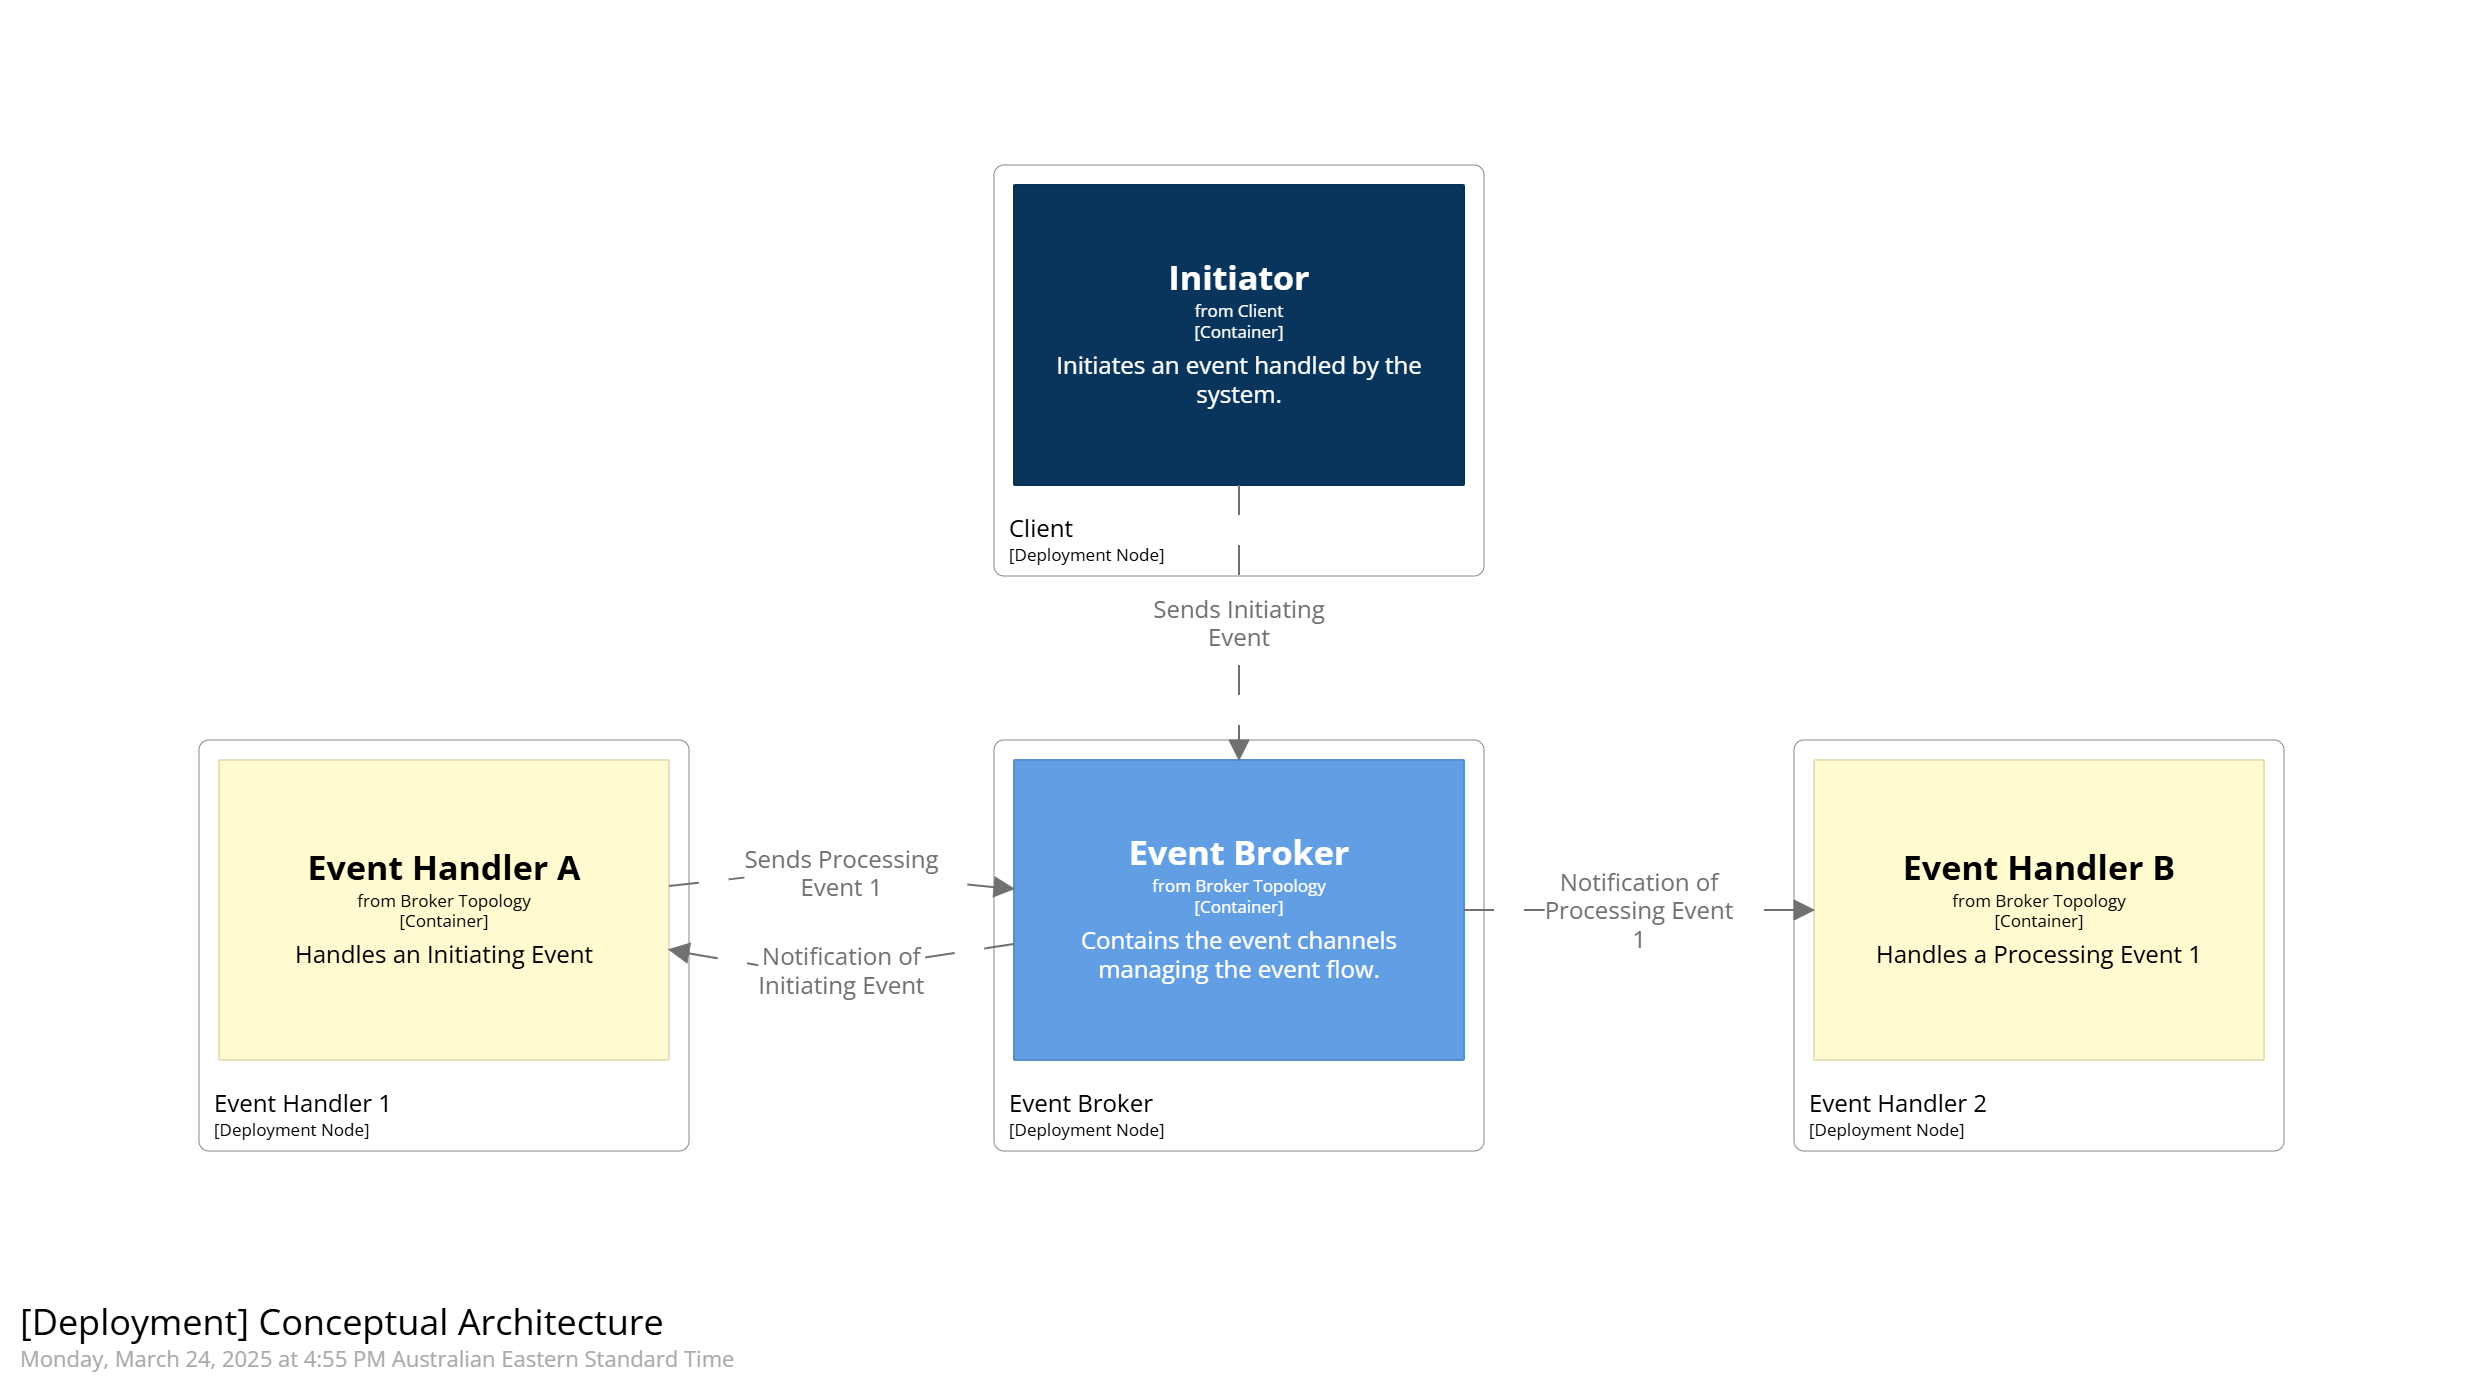
\includegraphics[trim=195 195 195 195,clip,width=0.97\paperwidth]{../../notes/event/diagrams/conceptual-architecture.png}
    \end{adjustwidth}
\end{frame}
\note{Comment on how each container is deployed in its own compute node.}

\begin{frame}{Terminology}
    \vspace{1mm}
    {\LARGE
    \begin{labeling}{Processing Event}
        \item<1->[\color{secondary} Initiating Event] Starts the business process
        \vspace{3mm}
        \item<2->[\color{secondary} Processing Event] Indicates next step in the process can be performed
        \vspace{3mm}
        \item<3->[\color{secondary} Event Channel] Holds events waiting to be processed
        \vspace{3mm}
        \item<4->[\color{secondary} Event Handler] Processes an event
        \begin{itemize}
            \Large\item Step, or part of a step, in the business process
        \end{itemize}
    \end{labeling}
    }
\end{frame}

\begin{frame}{Auction Example}
    \begin{adjustwidth}{-10mm}{-10mm}
        \centering
        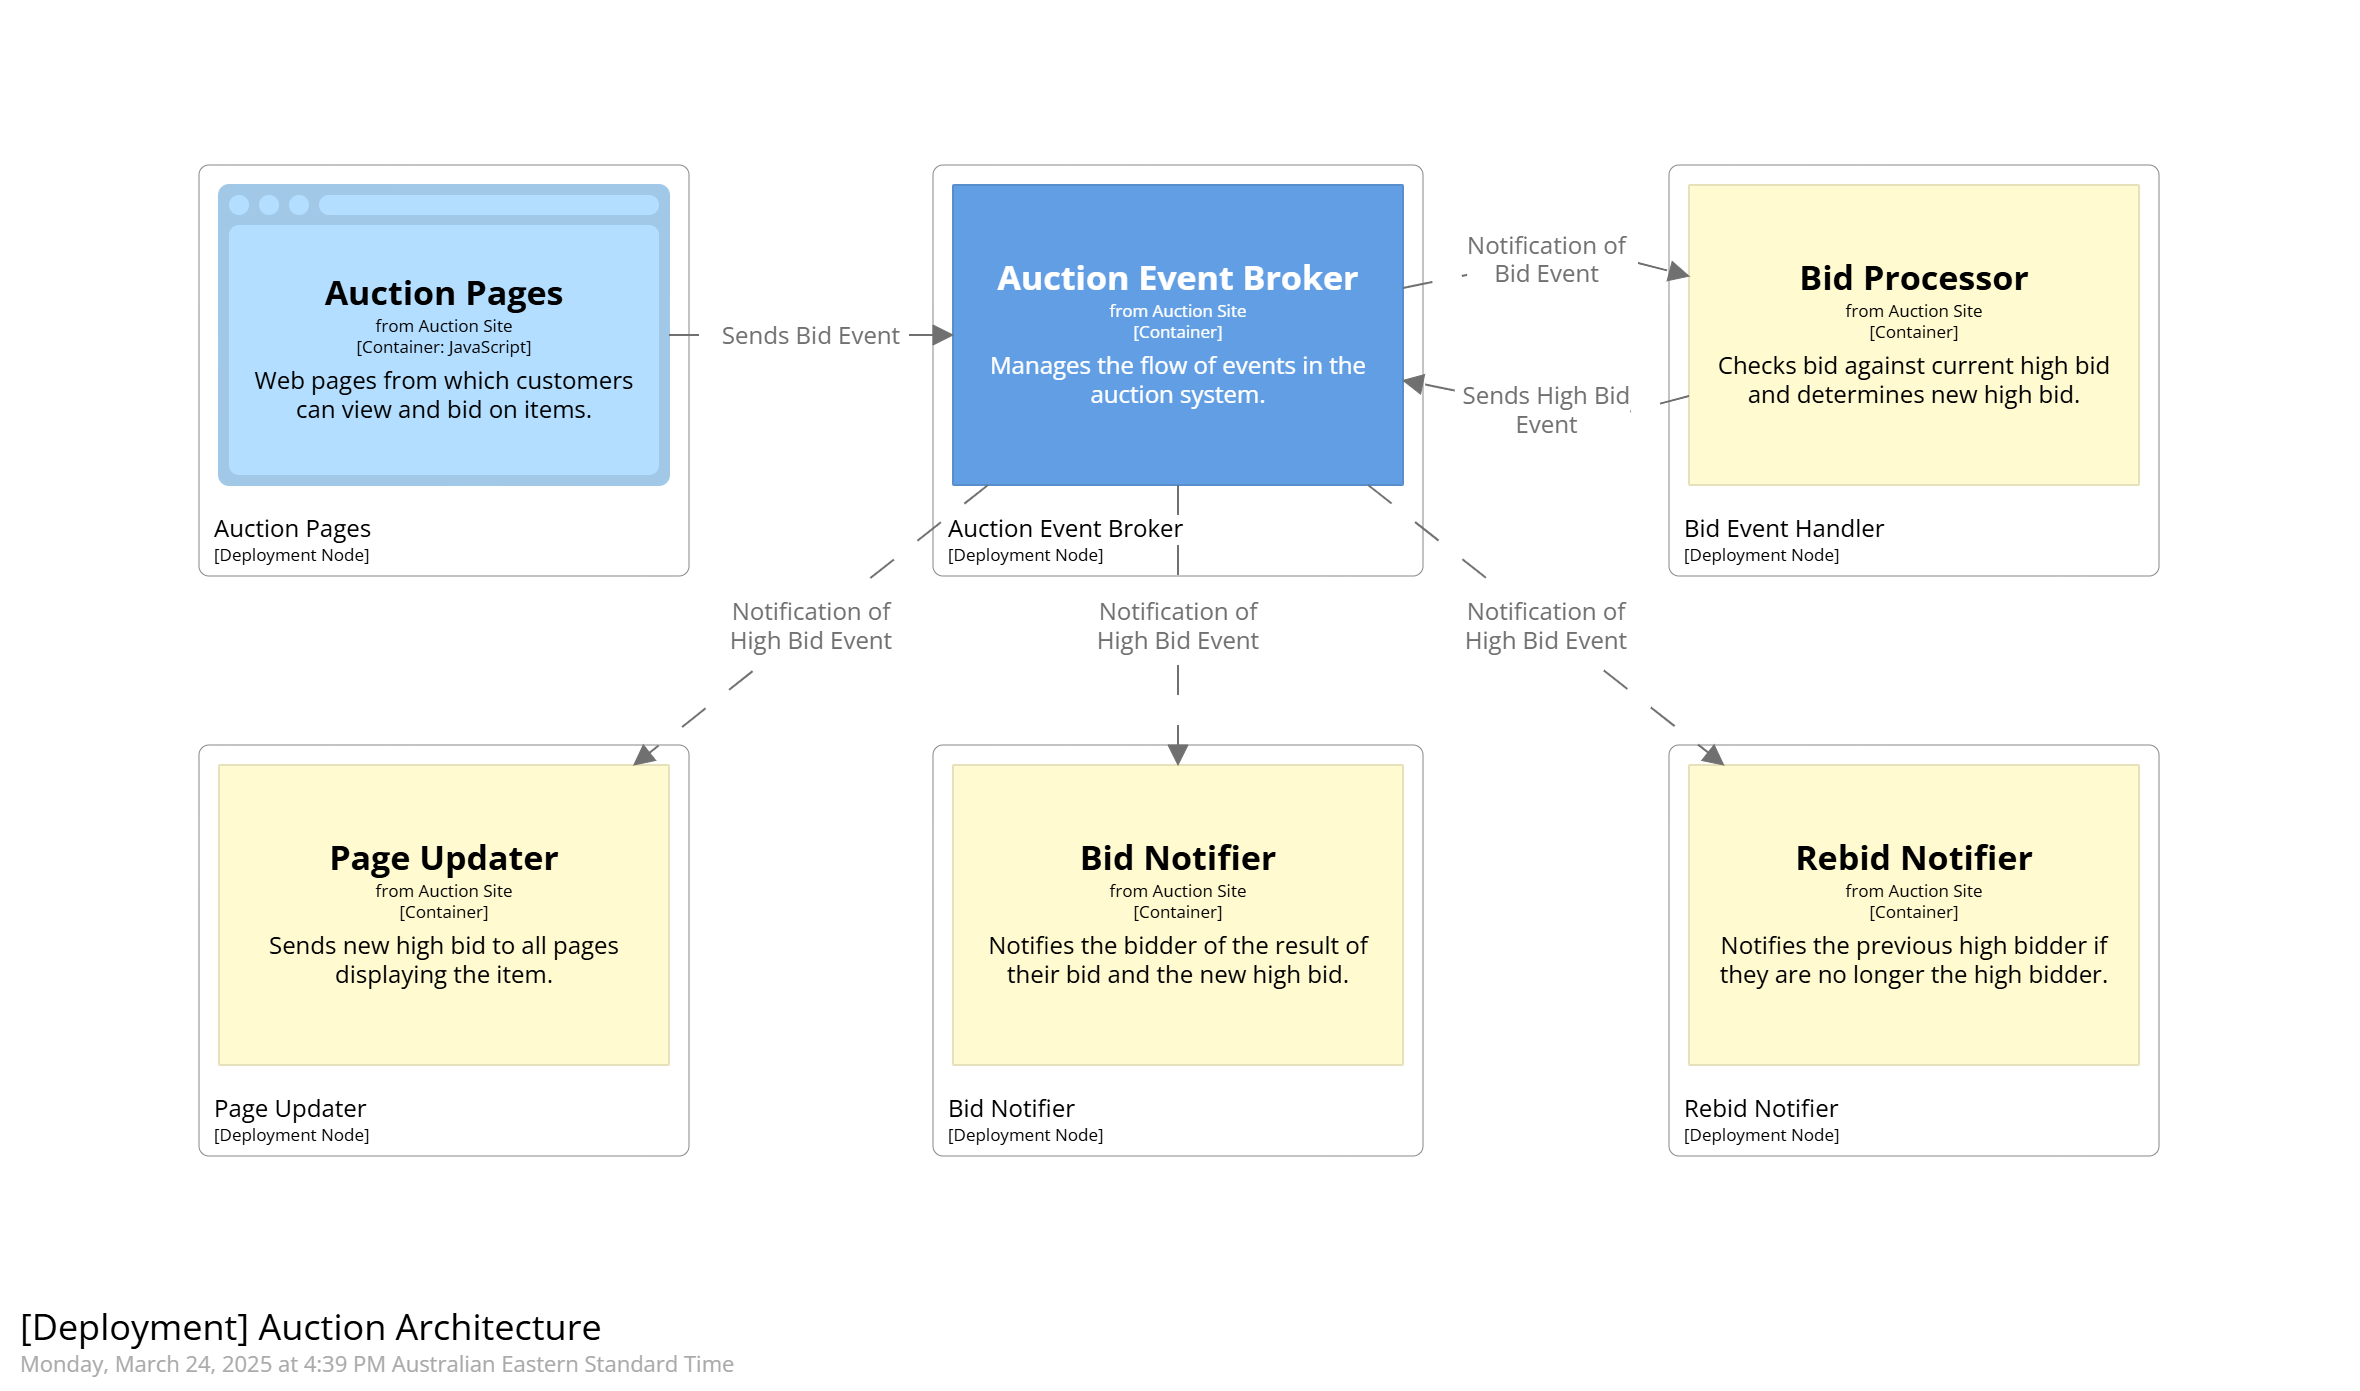
\includegraphics[trim=195 195 195 195,clip,width=0.97\paperwidth]{../../notes/event/diagrams/auction-architecture.png}
    \end{adjustwidth}
\end{frame}
\note[itemize]{
    \item Auction Event Broker has an API Gateway component to receive client requests and components to manage the event channels.
    \item Step through event process.
    \item Highlight asynchronous messages and parallel processing.
    \item Bid Processor could send back a high bid event or an async message.
}

\definition{Event Handler Cohesion Principle}
{Each event handler is a simple cohesive unit that performs a \highlight{single} processing task.}

\definition{Event Handler Independence Principle}
{Event handlers should not depend on the \highlight{implementation} of any other event handler.}

\begin{frame}{Auction Example -- Error Handling}
    \begin{adjustwidth}{-10mm}{-10mm}
        \centering
        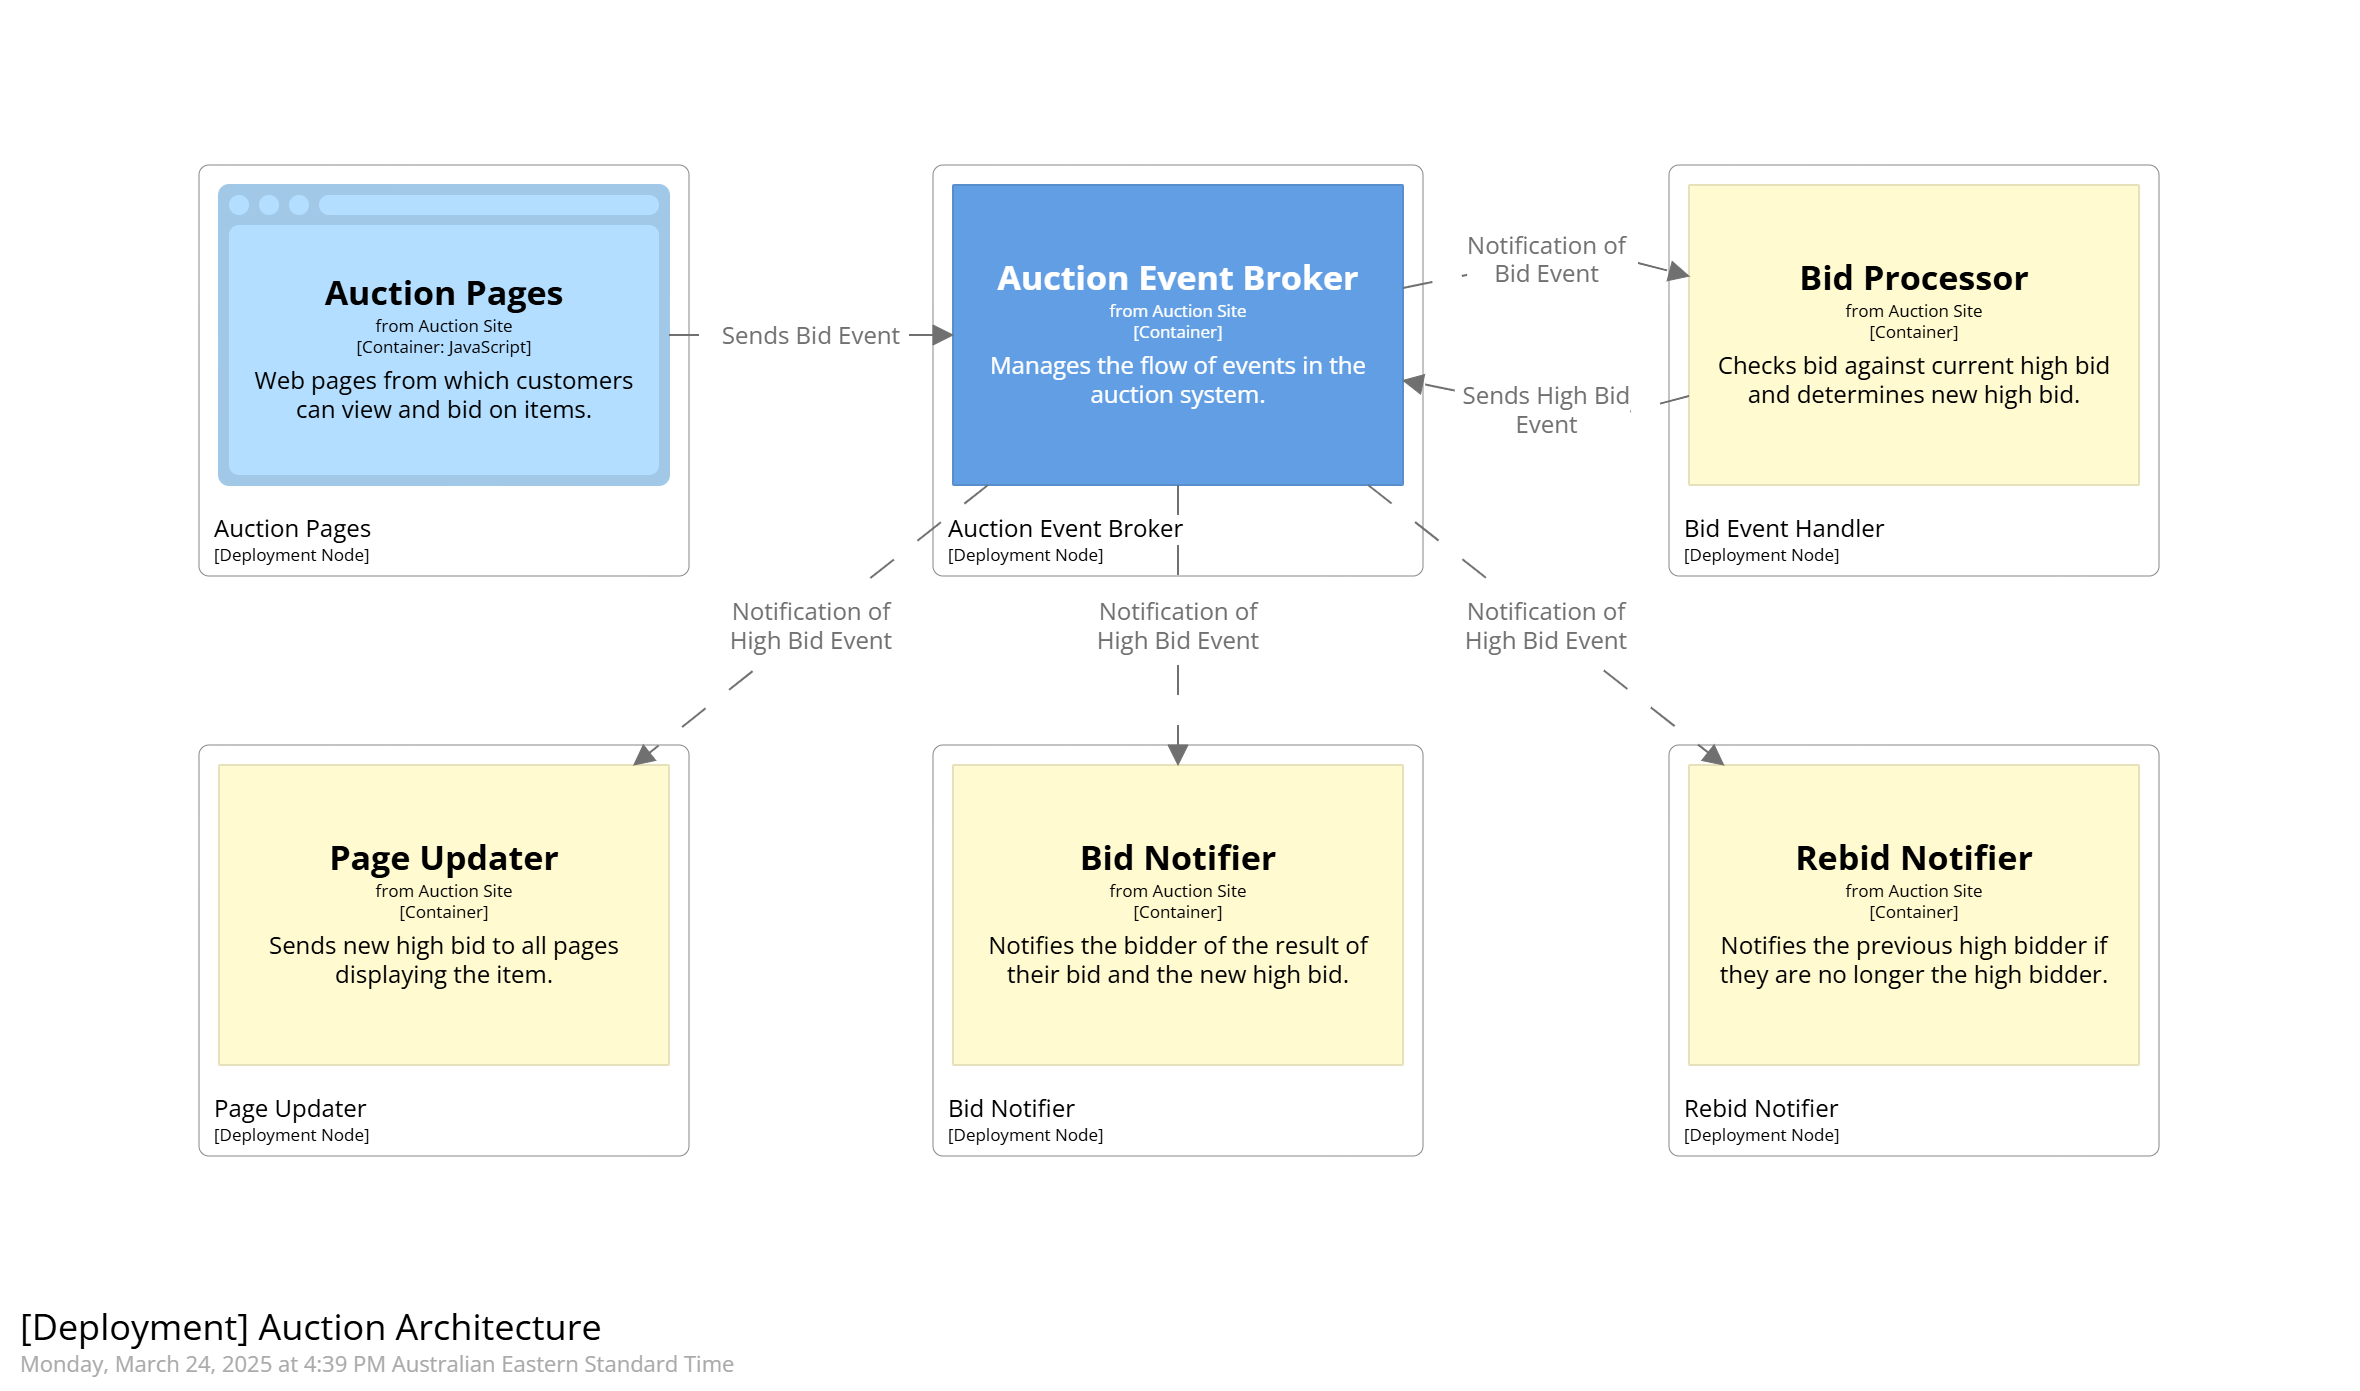
\includegraphics[trim=195 195 195 195,clip,width=0.97\paperwidth]{../../notes/event/diagrams/auction-architecture.png}
    \end{adjustwidth}
\end{frame}
\note[itemize]{
    \item How to handle Bid Processor failing?
    \item How to handle Rebid Notifier failing?
    \item How to handle Event Broker failing?
}

\begin{frame}{Topologies}
    \vspace{1mm}
    {\LARGE
    \begin{description}
        \item[Broker] All events received by event broker
        \begin{itemize}
            \Large\item Notifies event handlers of events
            \Large\item Event handlers send processing events when they finish processing
        \end{itemize}
        \vspace{3mm}
        \item[Mediator]<2-> Manages business process
        \begin{itemize}
            \Large\item Event queue of initiating events
            \Large\item Event mediator sends processing events to event handlers
            \Large\item Event handlers send async messages to mediator to report process finished
	\end{itemize}
    \end{description}
    }
\end{frame}

\begin{frame}{Broker Topology}
    \begin{adjustwidth}{-10mm}{-10mm}
        \centering
        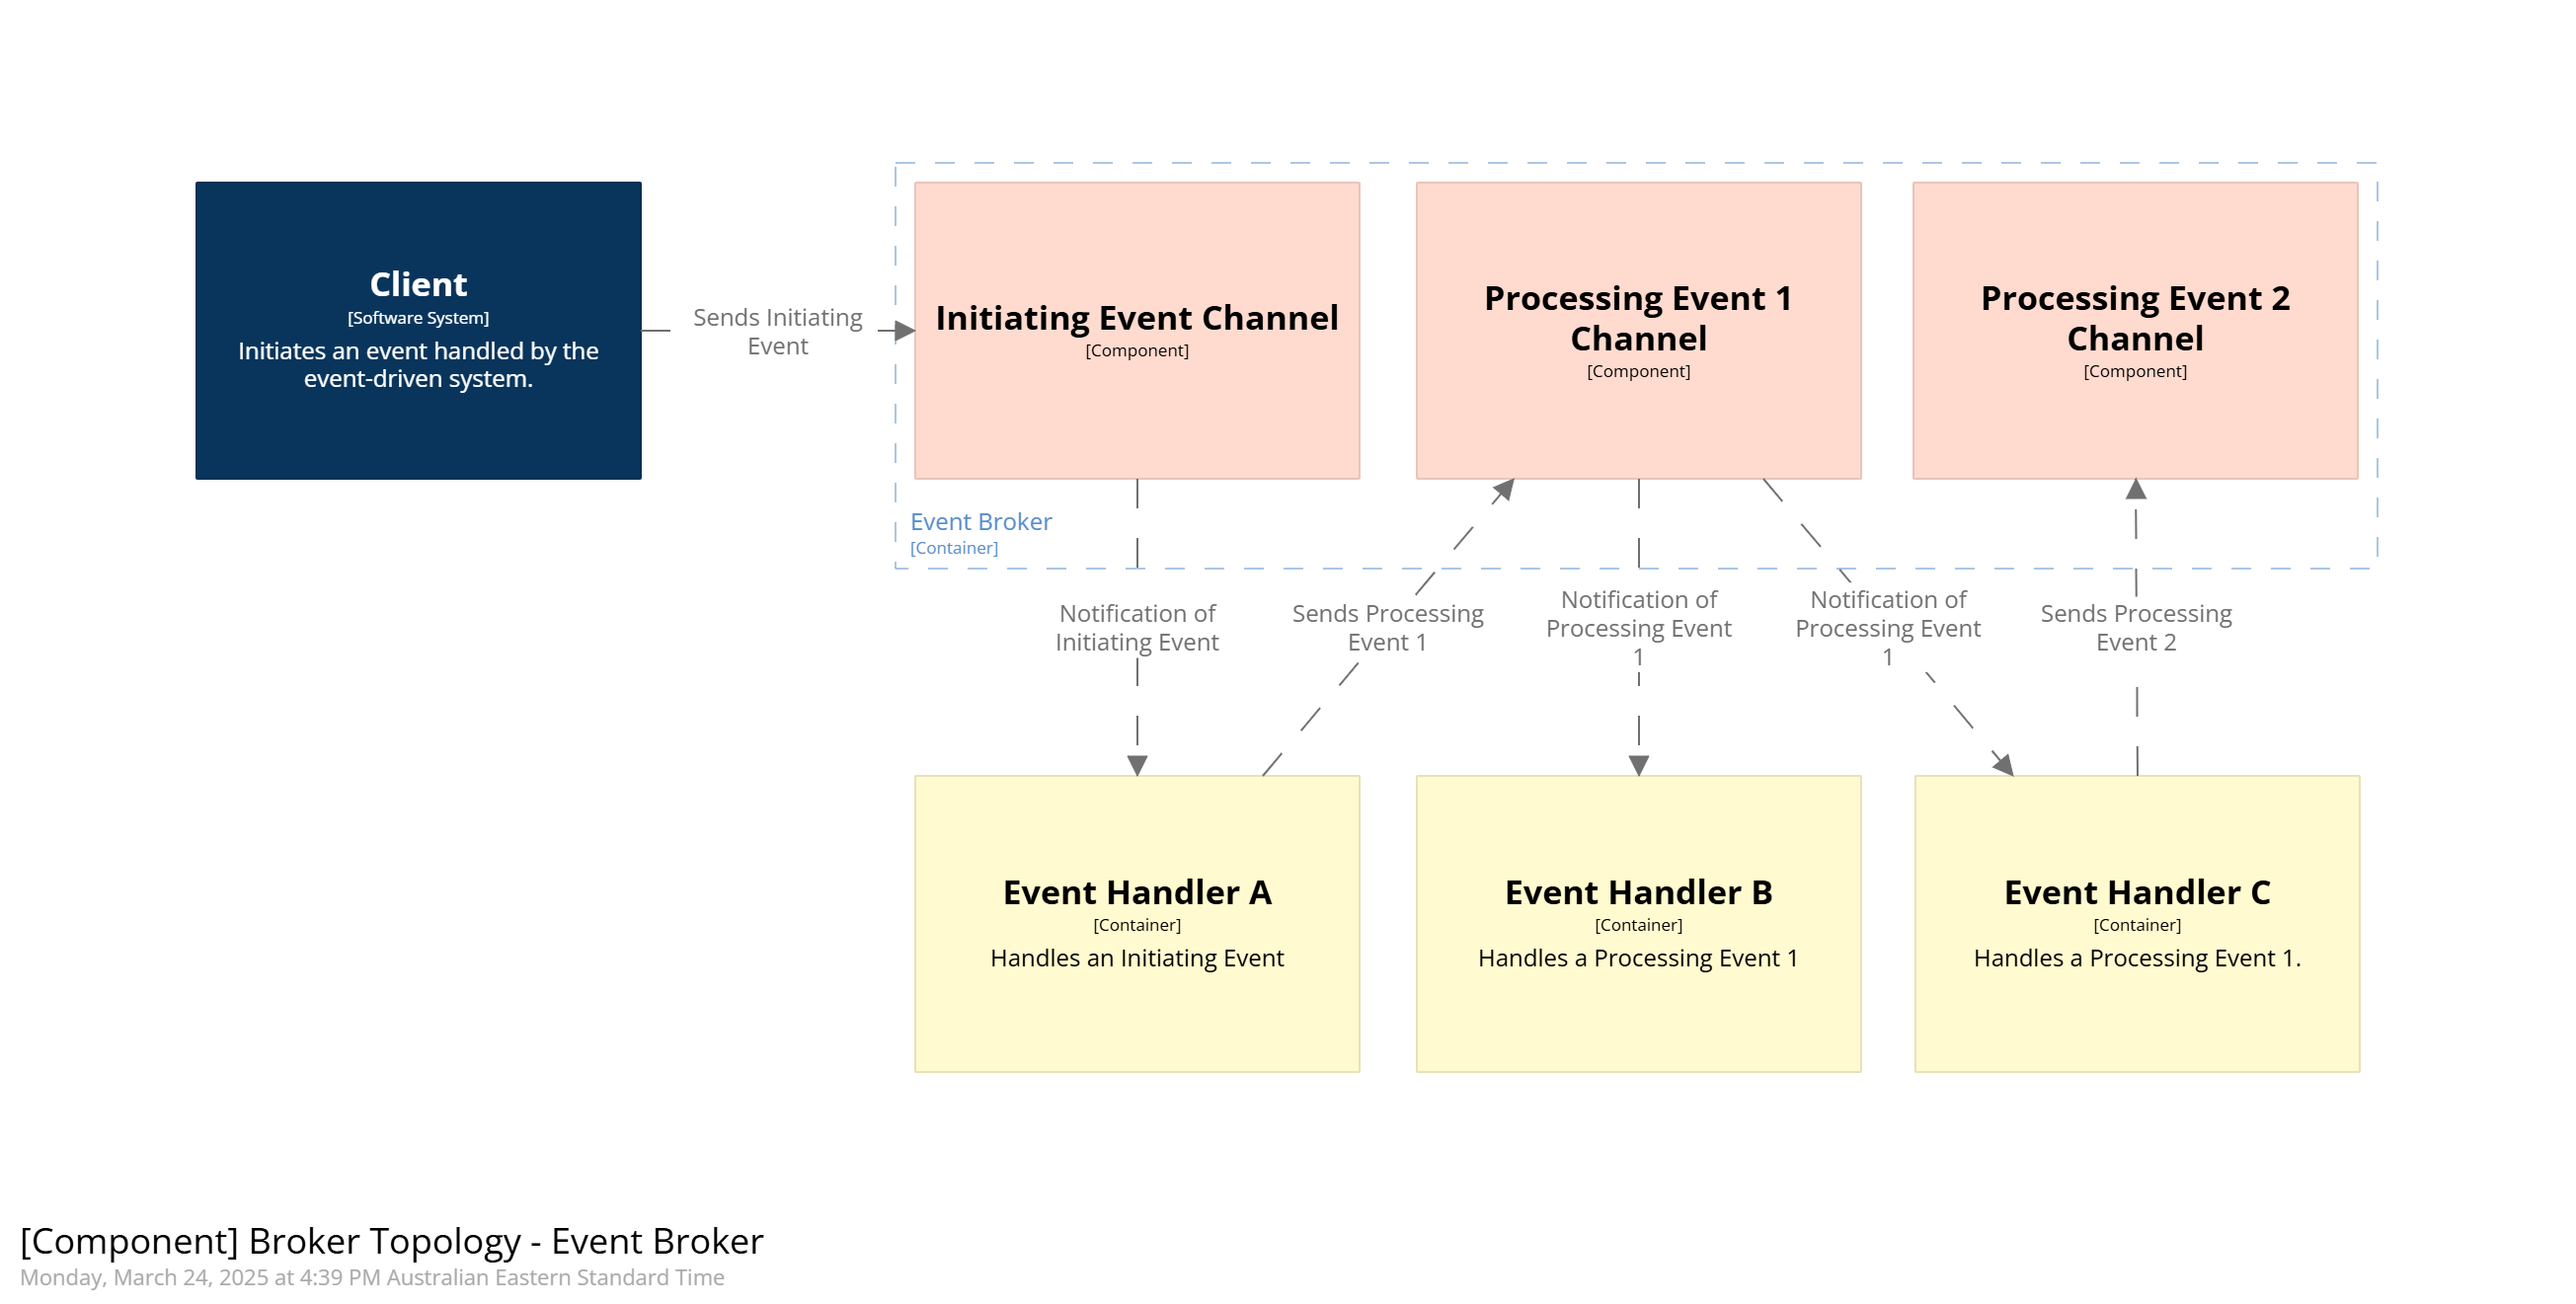
\includegraphics[trim=195 195 195 195,clip,width=0.97\paperwidth]{../../notes/event/diagrams/broker-components.png}
    \end{adjustwidth}
\end{frame}
\note[itemize]{
    \item Step through event process.
    \vspace{0.3em}
    \item Channels facilitate message flow.
    \begin{itemize}
        \item \large Commonly a lightweight message broker (e.g. RabbitMQ, ...).
    \end{itemize}
    \item Send final processing event, even if it is not handled.
    \begin{itemize}
        \item \large Easier to \highlight{extend} in the future.
    \end{itemize}
}

\point[\Large Event Broker Façade]{
\vspace{0.5em}
\begin{itemize}
    \item Event handlers register to \highlight{listen} for events
    \vspace{0.5em}
    \item Receives events and \highlight{directs} them to the correct channel
\end{itemize}
}

\begin{frame}{Broker with Façade Topology}
    \begin{adjustwidth}{-10mm}{-10mm}
        \centering
        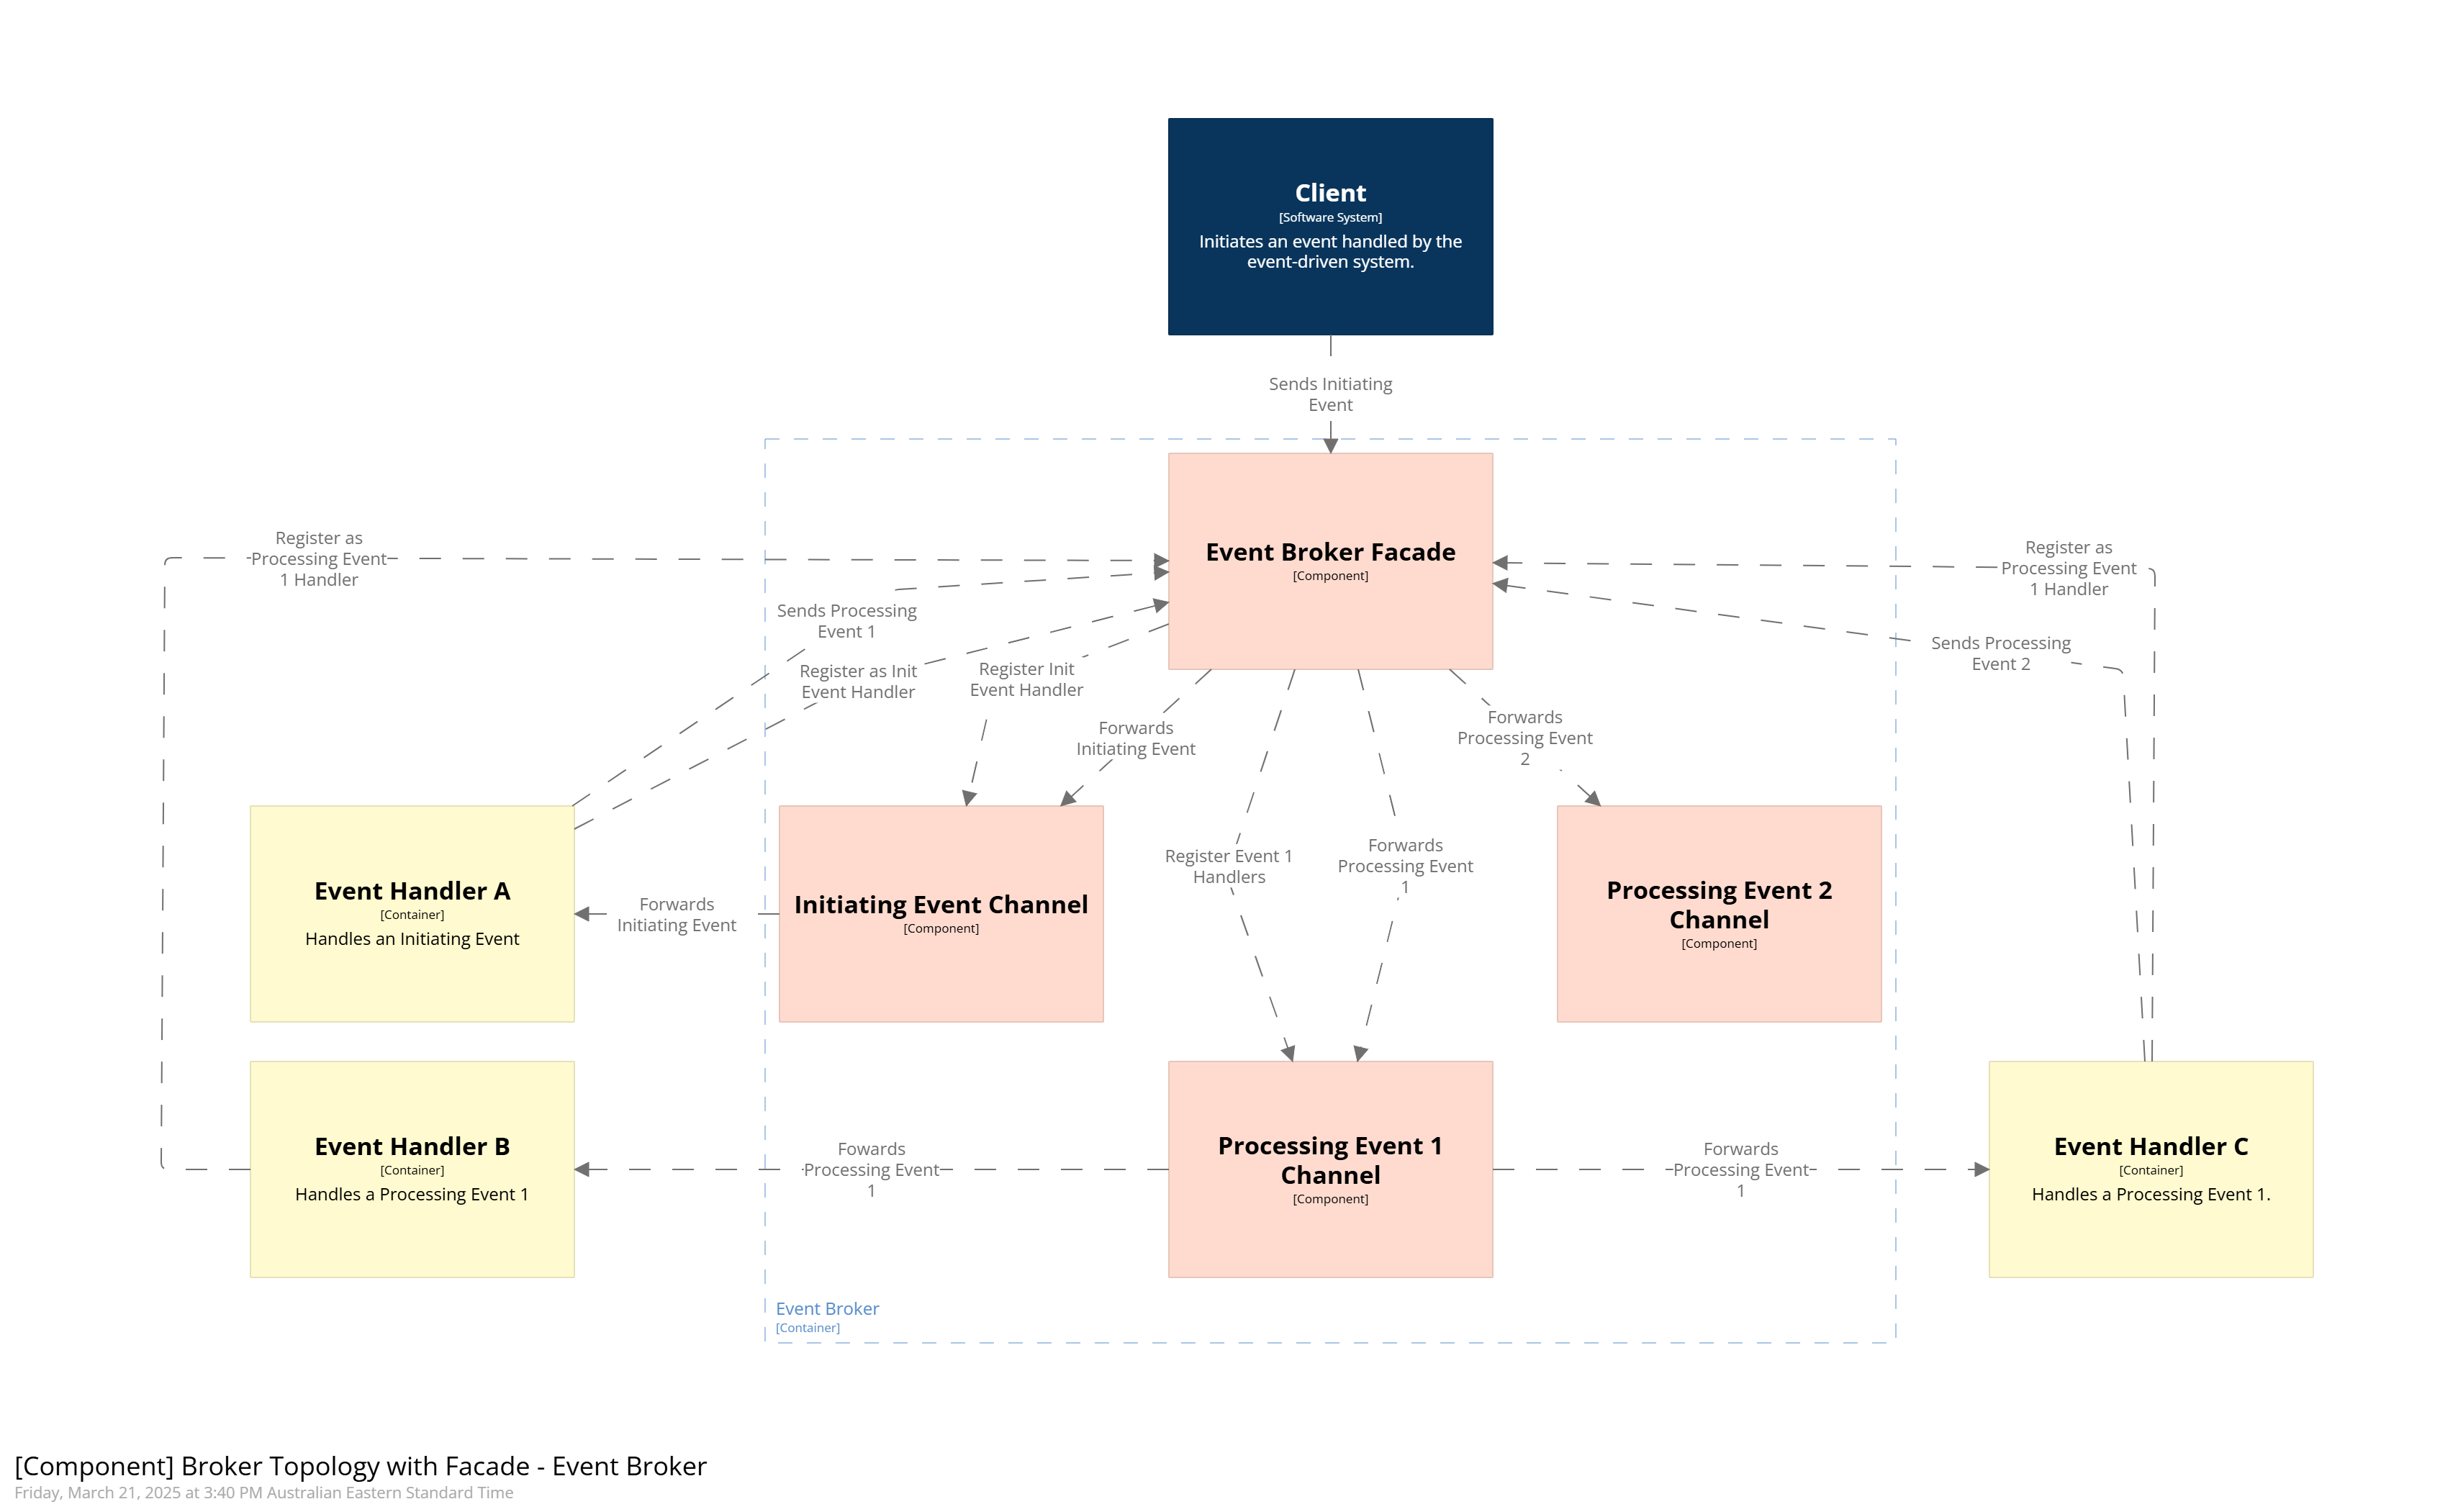
\includegraphics[trim=195 195 195 195,clip,width=0.91\paperwidth]{diagrams/broker-facade-components.png}
    \end{adjustwidth}
\end{frame}
\note[itemize]{
    \item Event processing \& event handling are the same.
    \vspace{0.4em}
    \item Now Event Handlers register, rather than being connected directly to Channels.
    \begin{itemize}
        \item \large Additional layer of abstraction.
    \end{itemize}
    \item Step through event process.
}

\begin{frame}{Mediator Topology}
    \begin{adjustwidth}{-10mm}{-10mm}
        \centering
        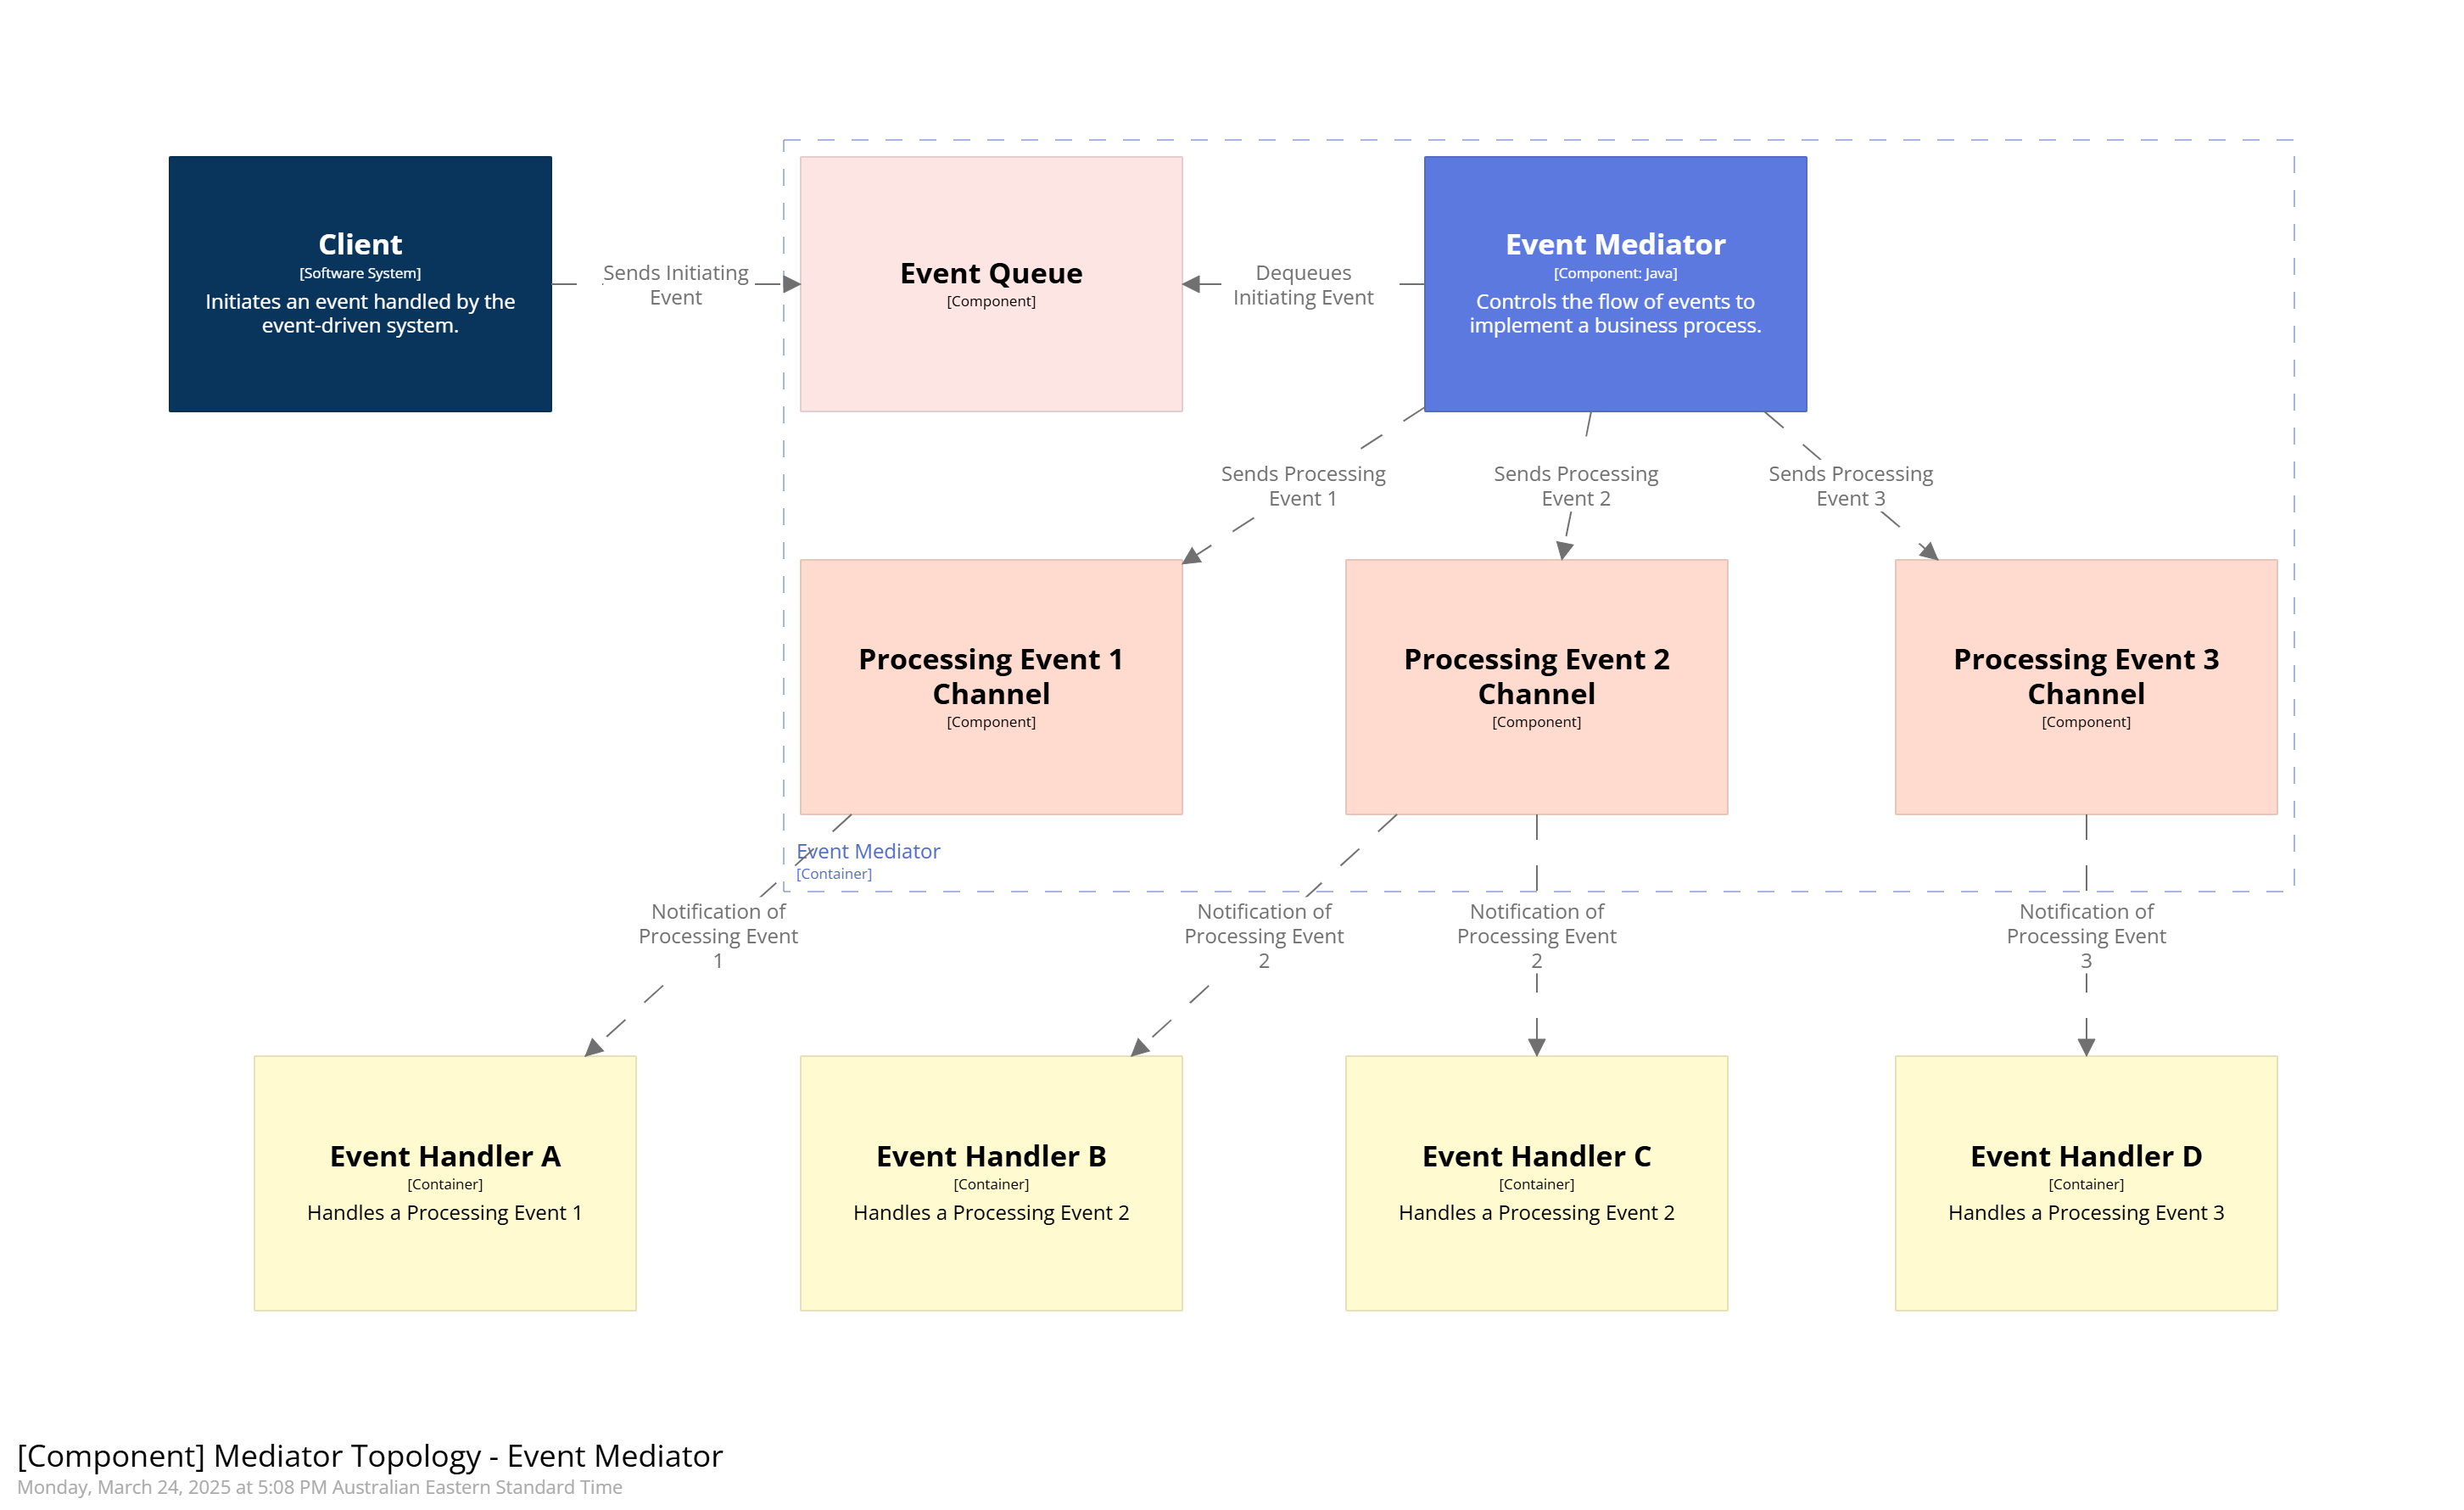
\includegraphics[trim=195 195 195 195,clip,width=1.43\paperheight]{../../notes/event/diagrams/mediator-components.png}
    \end{adjustwidth}
\end{frame}
\note[itemize]{
    \item Step through event process.
    \item Highlight process control performed by mediator.
}

\begin{frame}{Sahara Mediator Topology}
    \begin{adjustwidth}{-10mm}{-10mm}
        \centering
        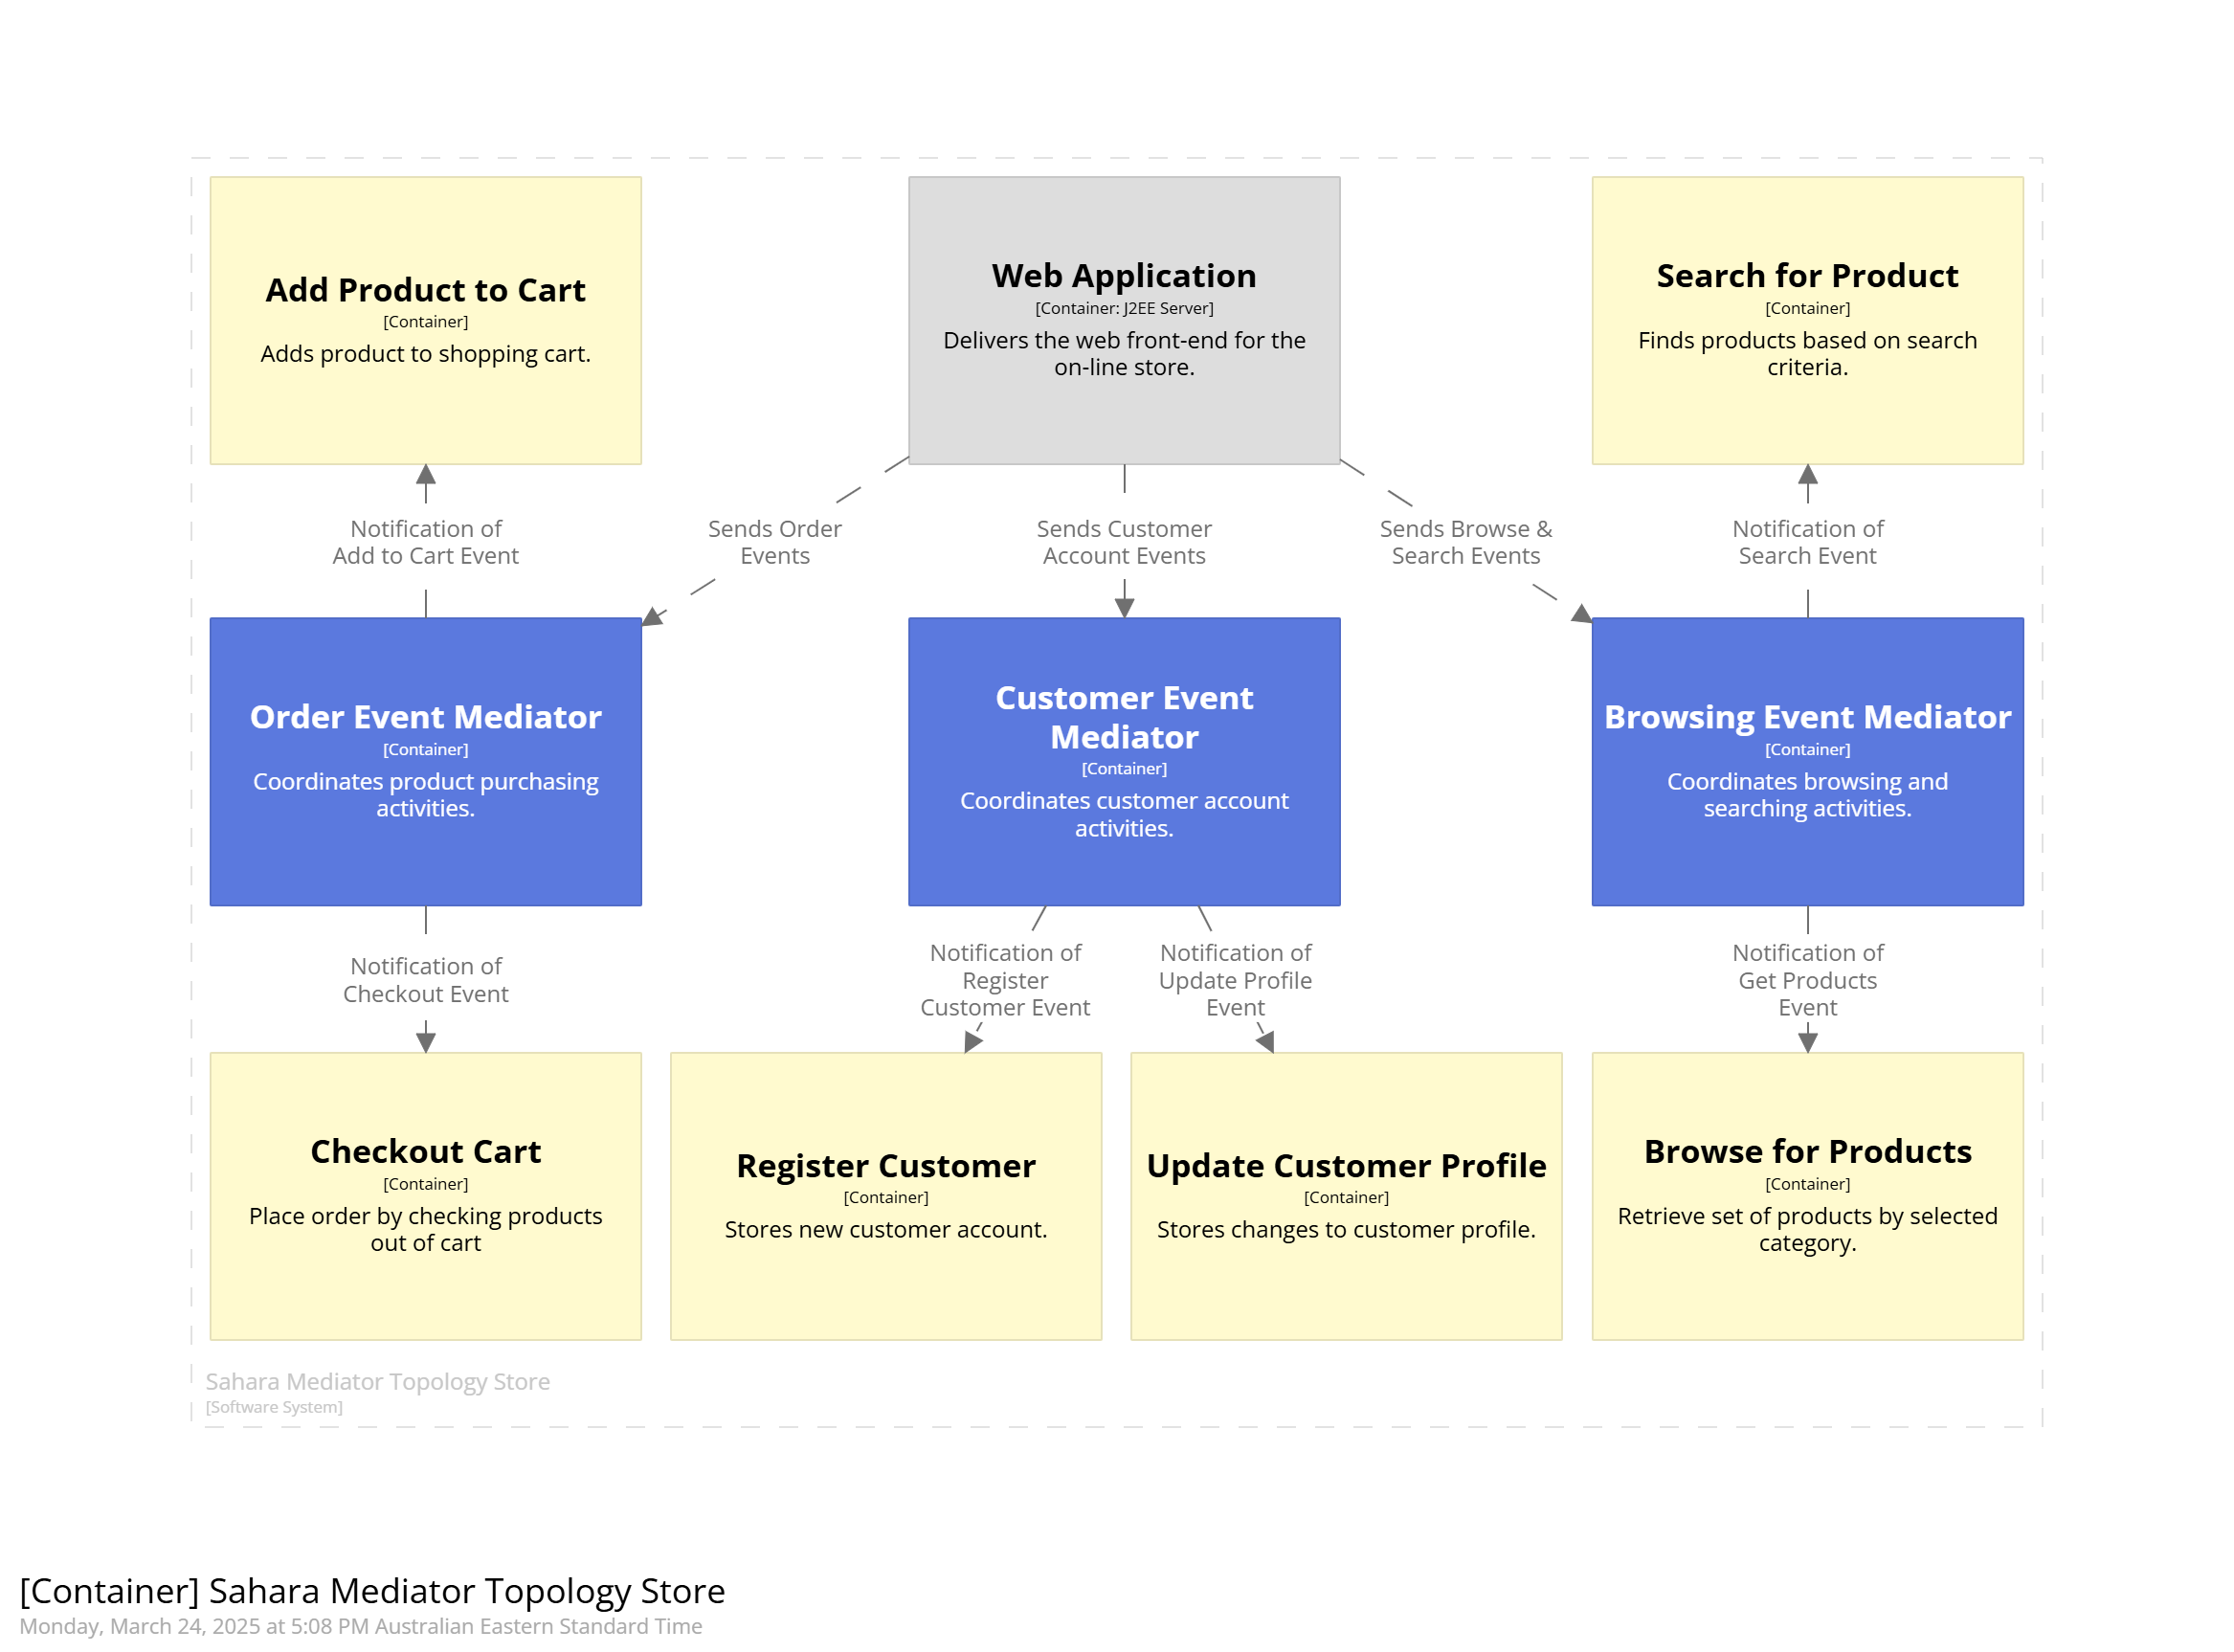
\includegraphics[trim=195 195 195 195,clip,width=0.69\paperwidth]{diagrams/sahara-mediator-container.png}
    \end{adjustwidth}
\end{frame}
\note[itemize]{
    \item Step through event process.
    \item Multiple mediators is common -- \highlight{one} per domain.
    \item Discuss internals of mediators: event queue and event channels.
}

%TODO Add component diagram showing internals of one mediator container.

\begin{frame}{Extensibility}
    \vspace{1mm}
    {\LARGE
    \begin{itemize}
        \item New behaviour for existing event
        {\vspace{1mm}\Large
        \begin{description}
            \item[Broker] Implement event handler \& register with broker
            \begin{itemize}
                \large\item Existing ignored event hooks
            \end{itemize}
            \item[Mediator] Implement event handler \& modify mediator logic
        \end{description}
	}
        \vspace{0.5em}
        \item<2-> New event
        {\Large
        \begin{description}
            \item[Broker] Implement event \& event handler, create event channel, modify broker façade
            \item[Mediator] Implement event \& event handler, modify mediator logic
	\end{description}
	}
    \end{itemize}
    }
\end{frame}


%TODO Add diagrams showing adding new event handler & adding new event to Broker topology.

%TODO Add diagrams showing adding new event handler & adding new event to Mediator topology.


\begin{frame}{Scalability}
    \vspace{1mm}
    {\LARGE
    \begin{itemize}
        \item Event handlers deployed independently
        \begin{itemize}
            \Large\item Scaled independently to manage load
        \end{itemize}
        \vspace{3mm}
        \item<2-> Event broker federated
        \begin{itemize}
            \Large\item Distributed across multiple compute nodes
        \end{itemize}
        \vspace{3mm}
        \item<3-> Event mediators for different domains
        \begin{itemize}
            \Large\item Distributes loads by domain\\(e.g. browse \& search, account, \& order events)
            \begin{itemize}
                \large\item Scaled independently to manage load
            \end{itemize}
        \end{itemize}
    \end{itemize}
    }
\end{frame}

\begin{frame}{Queues}
    \vspace{1mm}
    {\LARGE
    \begin{itemize}
        \item Channels can be implemented as queues
        \begin{itemize}
            \Large\item FIFO behaviour
        \end{itemize}
        \vspace{3mm}
        \item<2-> Multiple front of queue pointers
        \begin{itemize}
            \Large\item For each event handler
        \end{itemize}
        \vspace{3mm}
        \item<3-> Event removed when event handlers finish
        \begin{itemize}
            \Large\item Retry if a handler fails
        \end{itemize}
        \vspace{3mm}
        \item<4-> Events persist until removed
        \begin{itemize}
            \Large\item Recovery from broker failure
        \end{itemize}
    \end{itemize}
    }
\end{frame}

\begin{frame}{Streams}
    \vspace{1mm}
    {\LARGE
    \begin{itemize}
        \item Channels can be implemented as streams
        \begin{itemize}
            \Large\item Events are saved permanently
        \end{itemize}
        \vspace{3mm}
        \item<2-> Handlers notified when event added to stream
        \begin{itemize}
            \Large\item Observer pattern
        \end{itemize}
        \vspace{3mm}
        \item<3-> Handlers process events at their own pace
        \begin{itemize}
            \Large\item Cardiac arrest alarm vs. heart rate graph
        \end{itemize}
        \vspace{3mm}
        \item<4-> Events history
        \begin{itemize}
            \Large\item Redo processing
            \vspace{0.5mm}
            \Large\item Review processing activities
        \end{itemize}
    \end{itemize}
    }
\end{frame}

\begin{frame}{Queues vs Streams}
    \vspace{1mm}
    {\LARGE
    \begin{itemize}
        \item Queue
        \begin{itemize}
            \Large\item Known steps in business process
            \Large\item Easier sequencing of steps in business process
            \Large\item ``Exactly once'' semantics
            \Large\item eCommerce system
        \end{itemize}
        \vspace{3mm}
        \item<2-> Stream
        \begin{itemize}
            \Large\item Very large number of events or handlers
            \Large\item Handlers can ignore events
            \Large\item Analysis of past activity
            \Large\item Event sourcing
        \end{itemize}
    \end{itemize}
    }
\end{frame}

\begin{frame}{Broker vs Mediator Topologies}
    \vspace{1mm}
    {\LARGE
    \begin{description}
        \item[Broker] dumb pipe
        \vspace{3mm}
        \item[Broker] events have occurred
        \vspace{3mm}
        \item[Mediator]<2-> smart pipe
        \vspace{3mm}
        \item[Mediator]<2-> events are commands to process
    \end{description}
    }
\end{frame}

\begin{frame}{Broker vs Mediator Topologies}
    \vspace{1mm}
    \begin{columns}[t]
    \begin{column}{0.41\textwidth}
    {\LARGE
    \highlight{Broker Advantages}
    \begin{itemize}
        \item Scalability
        \item Reliability
        \item Extensibility
        \item Low coupling
    \end{itemize}
    }
    \end{column}
    \begin{column}{0.59\textwidth}
    {\onslide<2->\LARGE
    \highlight{Mediator Advantages}
    \begin{itemize}
        \item Complex business process logic
        \item Error handling
        \item Maintain process state
        \item Error recovery
    \end{itemize}
    }
    \end{column}
    \end{columns}
\end{frame}


\begin{frame}{Pros \& Cons}
    \vspace{1mm}
    {\LARGE
    \begin{description}
        \item[Modularity] Event Handlers \tabto{15em}\includegraphics[width=8mm]{../../shared/images/thumbs-up.png}
        \item[Extensibility] \tabto{15em}\includegraphics[width=8mm]{../../shared/images/thumbs-up.png}
        \item[Reliability] Event Handlers \tabto{15em}\includegraphics[width=8mm]{../../shared/images/thumbs-up.png}
        \item[Interoperability] Events \tabto{15em}\includegraphics[width=8mm]{../../shared/images/thumbs-up.png}
        \item[Scalability] Event Handlers \tabto{15em}\includegraphics[width=8mm]{../../shared/images/thumbs-up.png}
        \item[Security] \tabto{15em}\includegraphics[trim=57 145 70 85,clip,width=8mm]{../../shared/images/neutral.png}
        \item[Simplicity] \tabto{15em}\includegraphics[trim=22 19 22 12,clip,width=8mm]{../../shared/images/thumbs-down.png}
        \item[Deployability] \tabto{15em}\includegraphics[trim=22 19 22 12,clip,width=8mm]{../../shared/images/thumbs-down.png}
        \item[Testability] Complex Interactions \tabto{15em}\includegraphics[trim=22 19 22 12,clip,width=8mm]{../../shared/images/thumbs-down.png}
    \end{description}
    }
\end{frame}

\end{document}